% ============================================================
% WORK_TWELVE: Filtro adaptativo NLMS, comparacion contra LMS
% ============================================================

\subsection{WORK\_TWELVE: Filtro adaptativo NLMS}

Se implementó NLMS (Ec.~\ref{eq:nlms}) desde cero en
\texttt{nlms\_lab/adaptive.py}, de forma completamente independiente a
WORK\_ELEVEN —ninguno de los dos trabajos importa código del otro,
cada uno reimplementa localmente lo que necesita—, y se evaluó sobre
los mismos tres tipos de experimento usados para LMS, añadiendo además
una comparación directa entre ambos algoritmos bajo condiciones de
potencia de entrada no estacionaria.

\subsubsection{Identificación de sistema}

Sobre el mismo tipo de problema de identificación ciega de un filtro
FIR de 5 coeficientes excitado con ruido blanco descrito en la sección
anterior, NLMS partió de un error inicial de pesos de 0.9354 —el error
correspondiente a inicializar el vector de pesos en cero antes de
cualquier adaptación— y convergió a un error final prácticamente nulo
($\approx 10^{-6}$, Fig.~\ref{fig:work_twelve_t1}). La velocidad de
convergencia observada es comparable a la mejor región de LMS
(Sección~\ref{sec:resultados}, barrido de $\mu$), lo cual es esperable:
cuando la potencia de la señal de entrada es constante, el paso
efectivo de NLMS se estabiliza en un valor fijo y el algoritmo se
comporta de manera muy similar a LMS con un $\mu$ bien ajustado para
esa potencia particular. La diferencia entre ambos algoritmos solo se
hace evidente —y relevante en la práctica— cuando esa potencia deja de
ser constante, como se explora en la Sección~\ref{sec:nlms_vs_lms}.

\begin{figure}[!t]
\centering
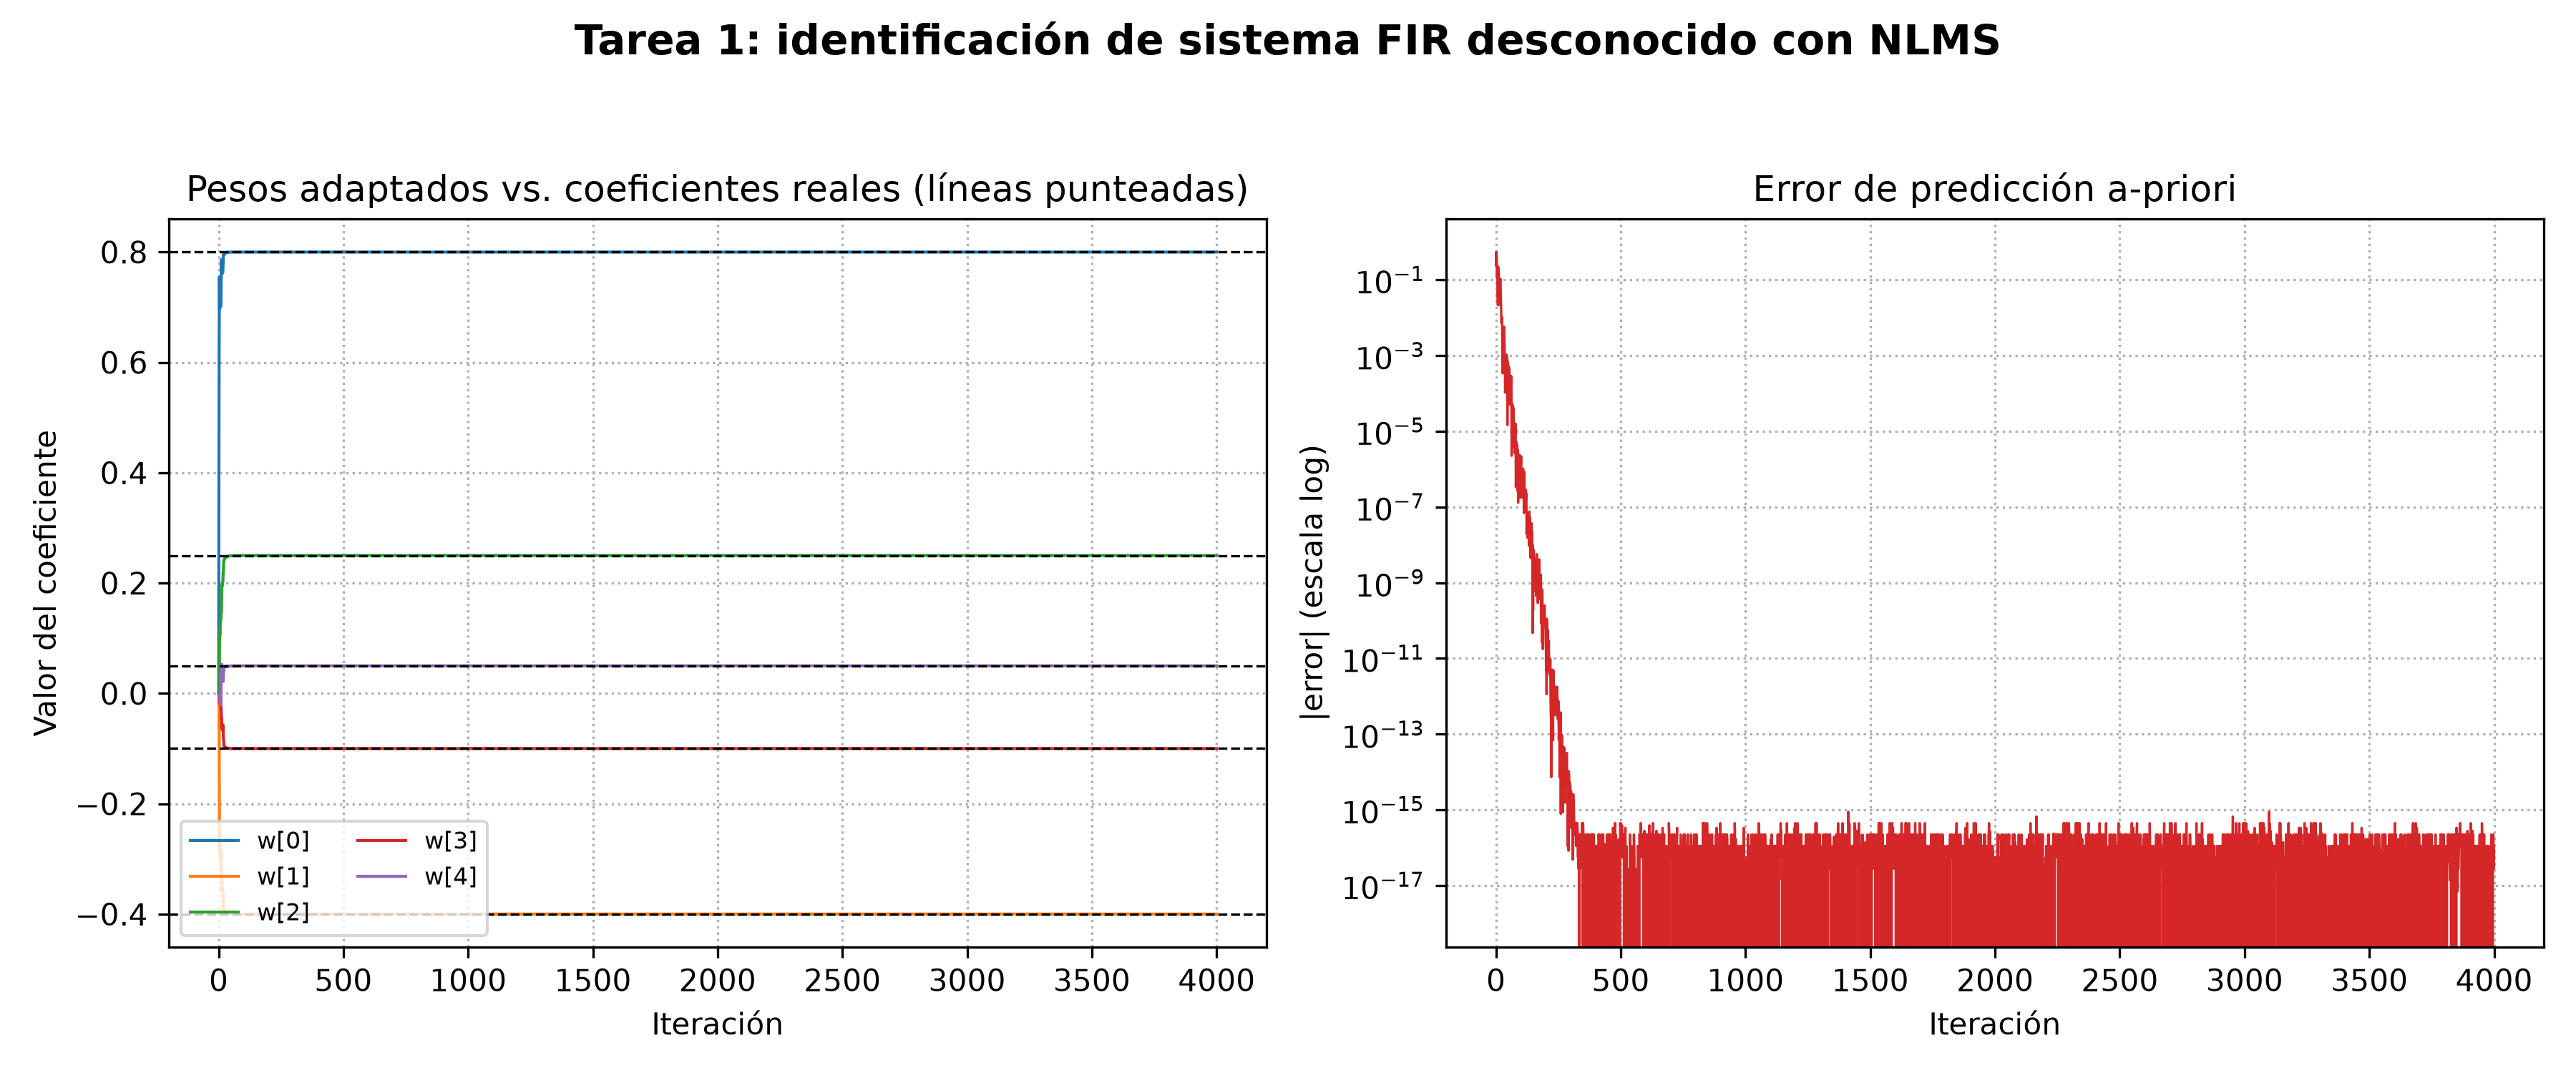
\includegraphics[width=\columnwidth]{work_twelve_t1_system_identification.png}
\caption{NLMS: convergencia de los pesos del filtro hacia los coeficientes reales del sistema FIR desconocido (panel superior) y evolución del error de identificación (panel inferior).}
\label{fig:work_twelve_t1}
\end{figure}

\subsubsection{Cancelación adaptativa de ruido}

Usando el mismo esquema de cancelación de ruido de dos entradas
descrito para LMS, NLMS recuperó tanto un tono sintético de 60~Hz como
la grabación de audio real contaminados con ruido correlacionado con
una señal de referencia. En el caso del tono, la desviación estándar
del residuo cayó de 0.5036 antes del filtrado a 0.1614 después —una
reducción de aproximadamente 3.1 veces en desviación estándar, del
mismo orden de magnitud que la obtenida con LMS bajo condiciones de
potencia constante, lo cual es consistente con la expectativa teórica
de que ambos algoritmos deberían comportarse de forma comparable
cuando no hay variación de potencia que explotar
(Fig.~\ref{fig:work_twelve_t2a}, \ref{fig:work_twelve_t2b}).

\begin{figure}[!t]
\centering
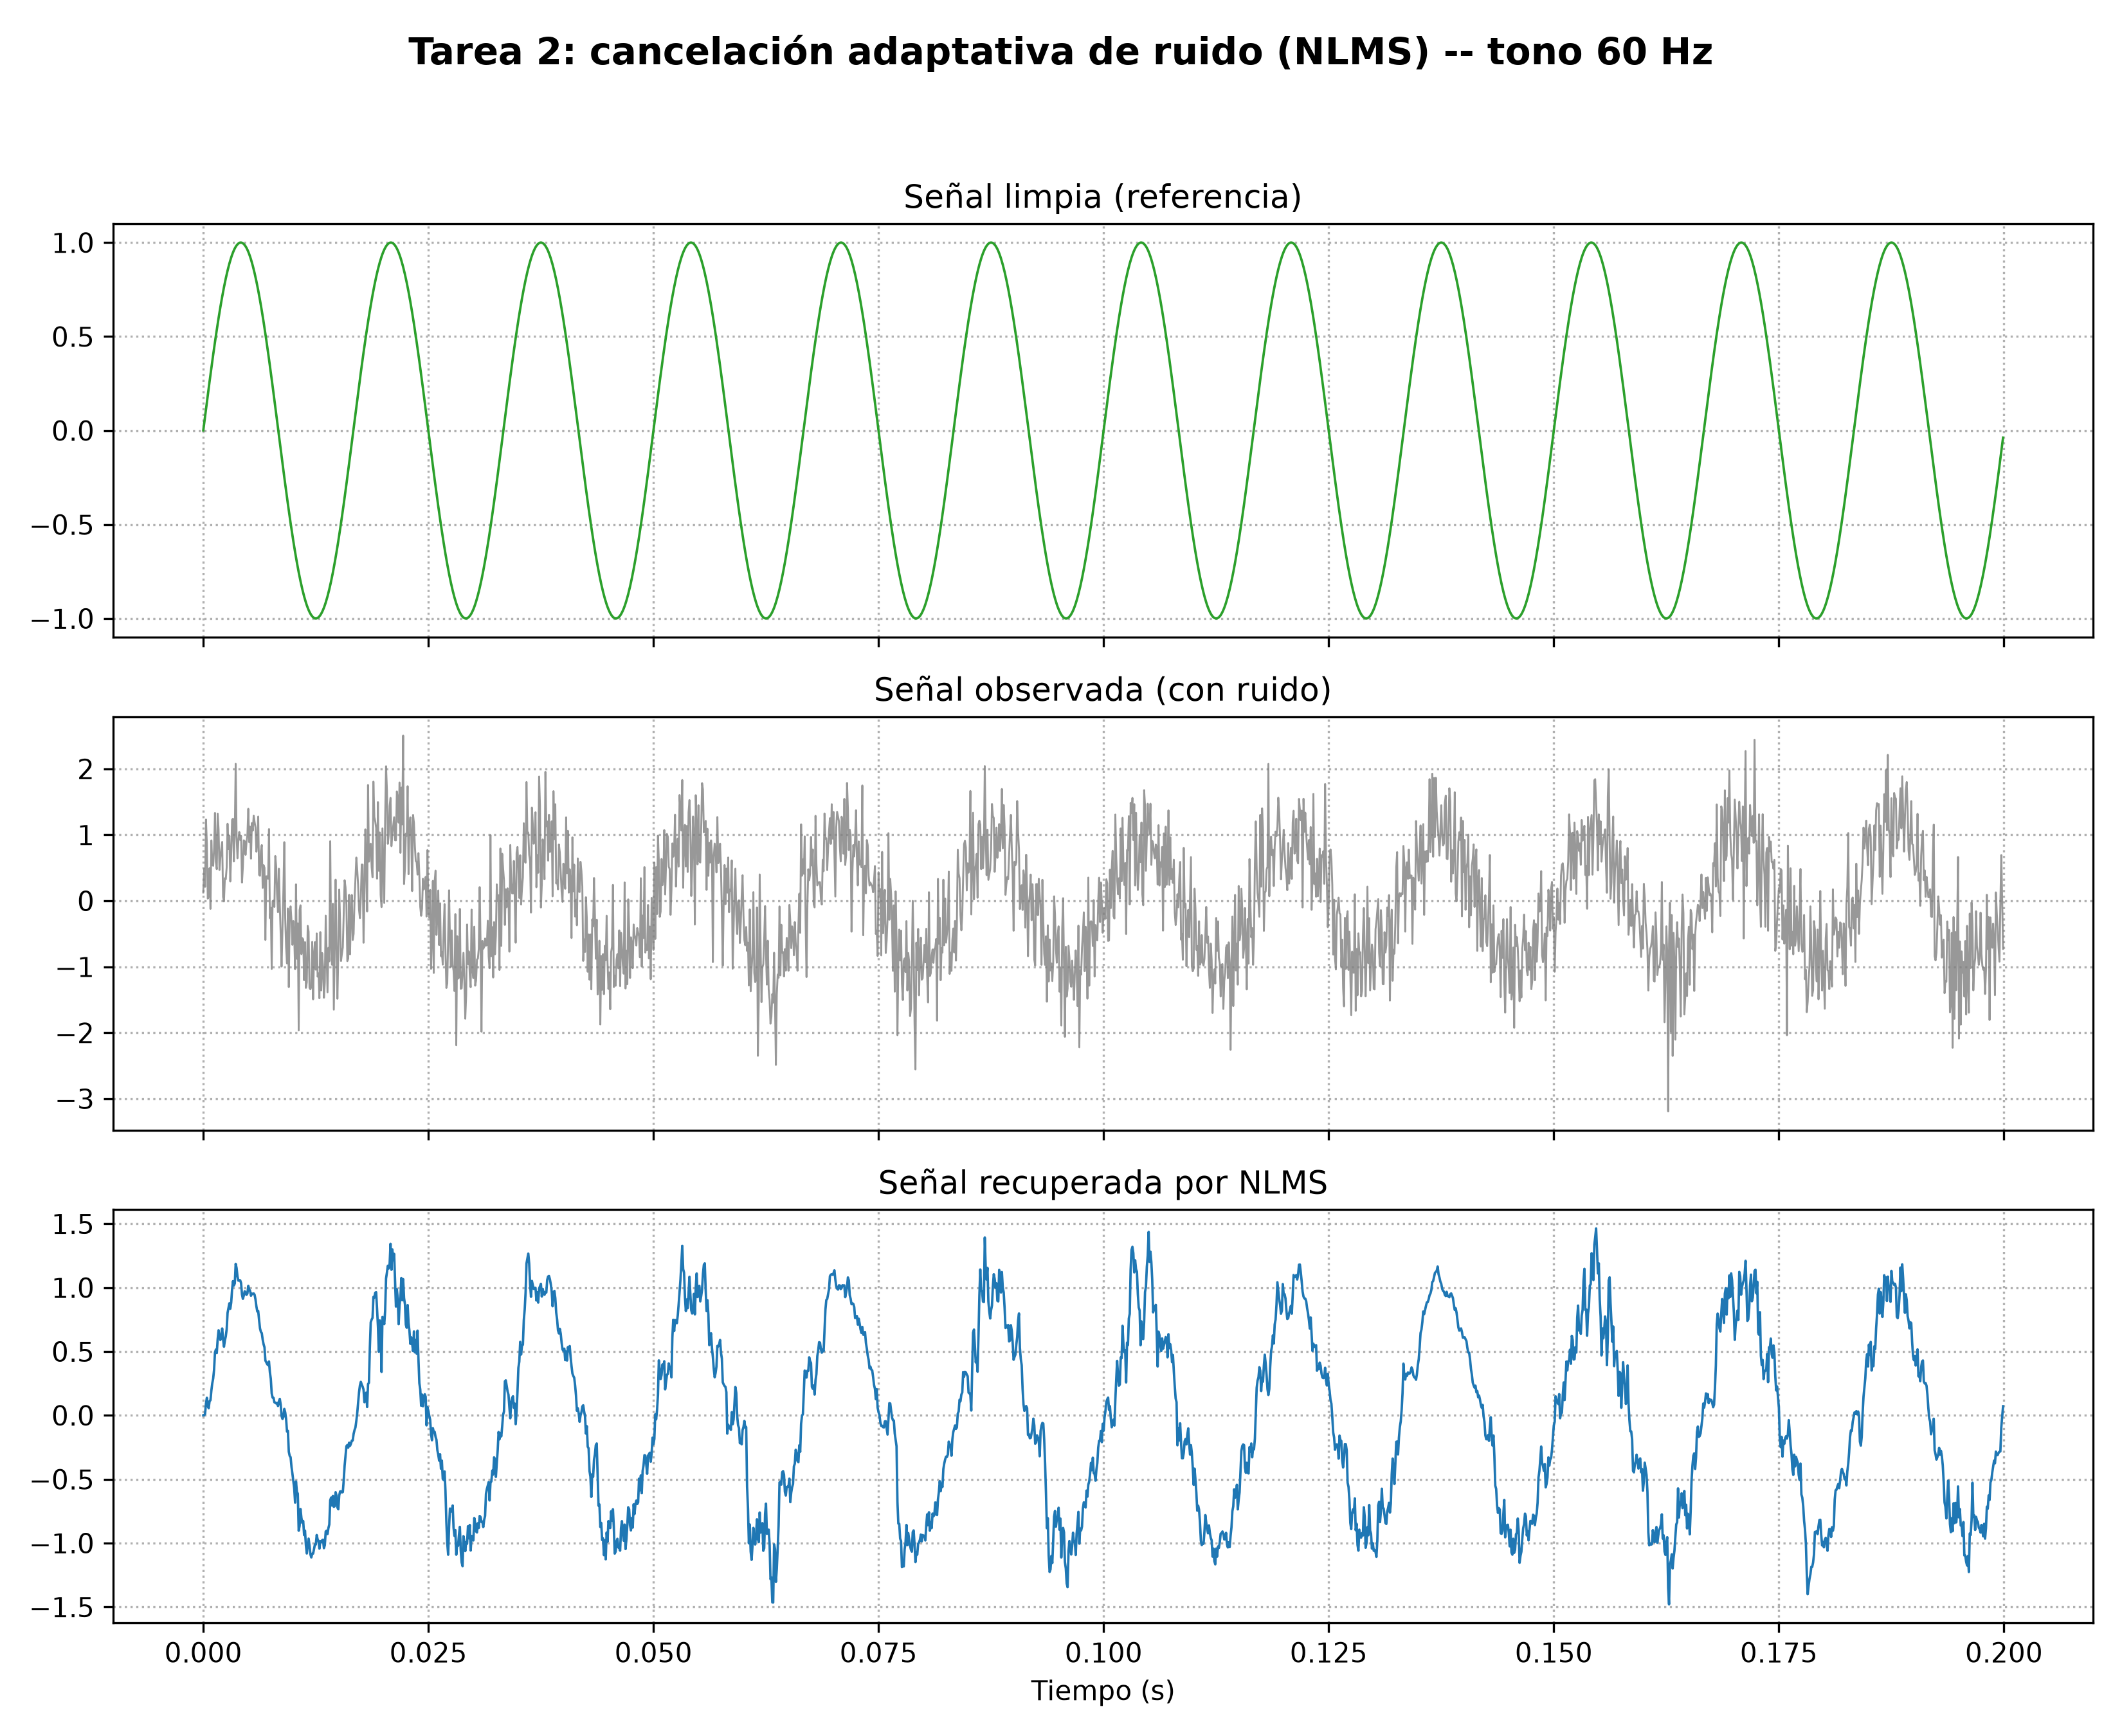
\includegraphics[width=\columnwidth]{work_twelve_t2_noise_cancellation_tone.png}
\caption{NLMS: cancelación adaptativa de ruido sobre un tono de 60~Hz.}
\label{fig:work_twelve_t2a}
\end{figure}

\begin{figure}[!t]
\centering
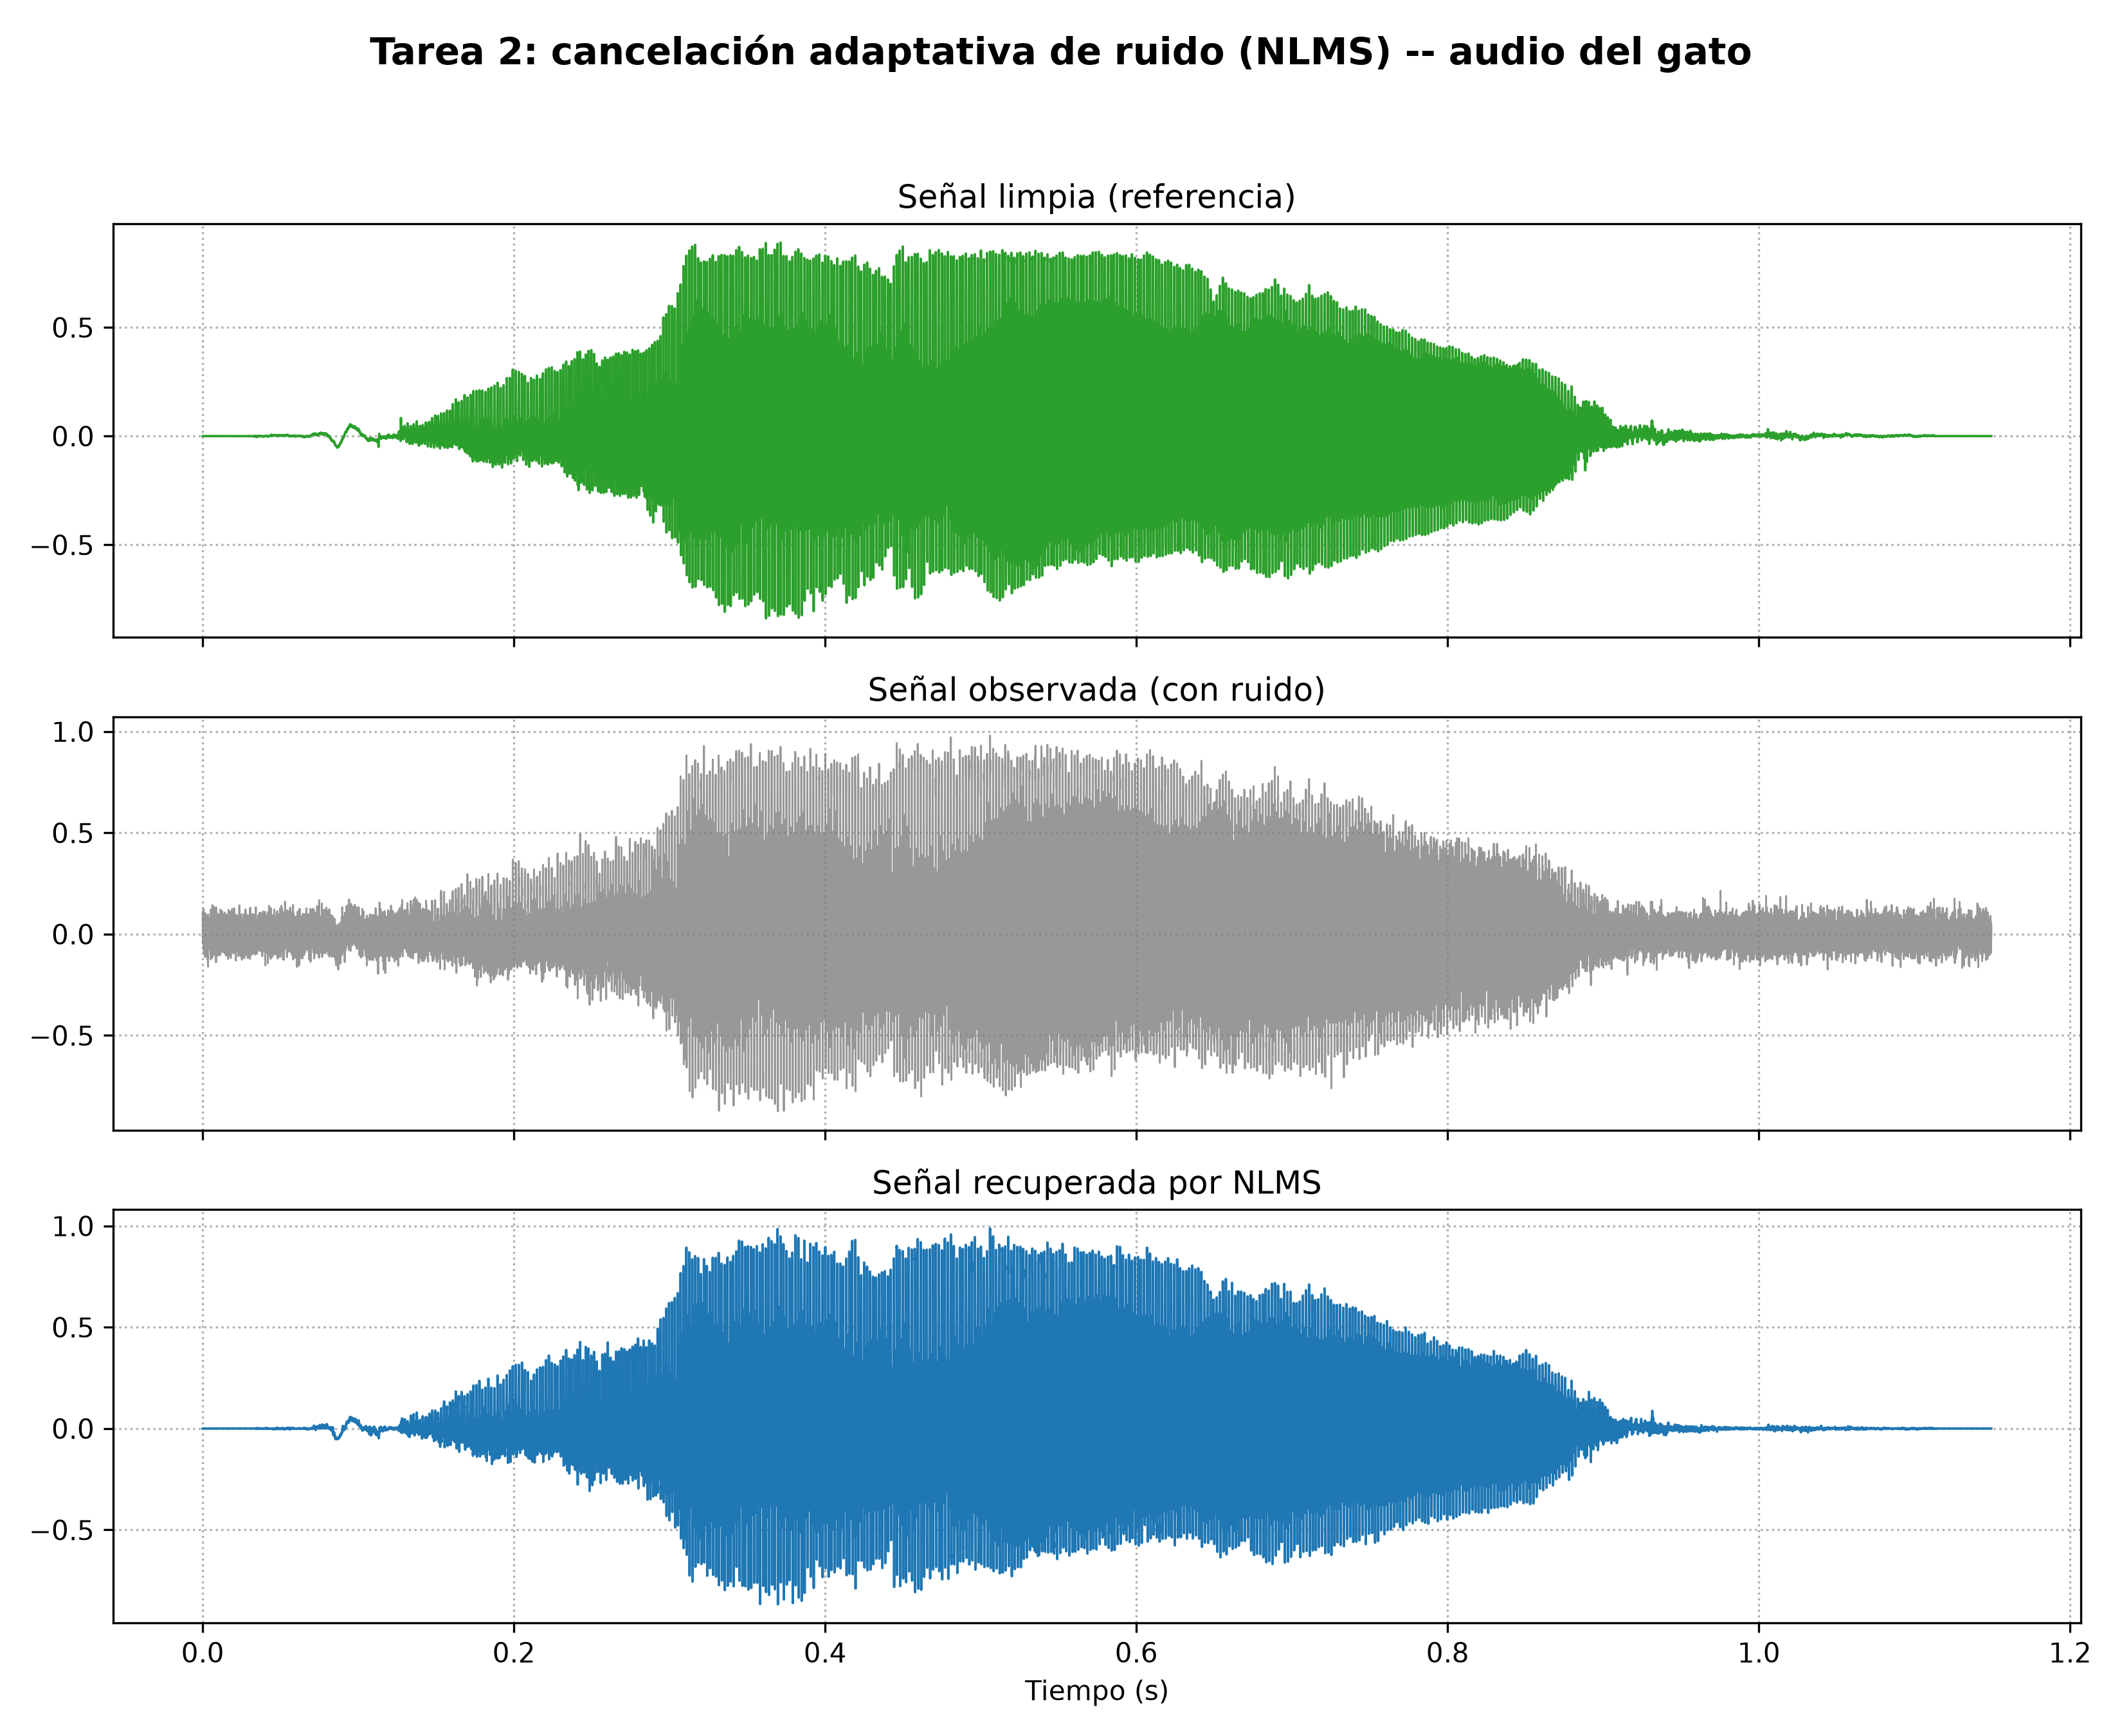
\includegraphics[width=\columnwidth]{work_twelve_t2_noise_cancellation_cat.png}
\caption{NLMS: cancelación adaptativa de ruido sobre una grabación de audio real.}
\label{fig:work_twelve_t2b}
\end{figure}

\subsubsection{NLMS frente a LMS bajo potencia de entrada no estacionaria}
\label{sec:nlms_vs_lms}

El experimento más relevante de este trabajo busca exponer, de forma
cuantitativa y no solo cualitativa, la ventaja práctica que justifica
preferir NLMS sobre LMS en aplicaciones reales. Para ello se repitió el
problema de identificación de sistema con una señal de entrada cuya
amplitud cambia abruptamente por un factor de 40 a la mitad del
experimento —simulando, de forma simplificada, el tipo de variación de
potencia que aparece en señales de voz (pasajes hablados frente a
silencios) o en canales de comunicación con desvanecimiento. Se
comparó NLMS contra una reimplementación local de LMS con un único
valor de $\mu$, fijo durante todo el experimento y elegido
deliberadamente para que el filtro se mantenga estable durante el
segmento de \emph{mayor} potencia —la elección natural que haría un
diseñador que solo puede fijar un parámetro antes de observar cómo se
comportará la señal en el tiempo.

Los resultados (Fig.~\ref{fig:work_twelve_t3}) muestran una diferencia
sustancial: en el segmento de \emph{menor} potencia, el error cuadrático
medio en estado estacionario de LMS fue de 0.03967, frente a 0.00117
para NLMS —es decir, LMS mantiene un error aproximadamente 34 veces
mayor que NLMS bajo las mismas condiciones de entrada y el mismo
sistema desconocido a identificar. La razón es exactamente la prevista
por la teoría: el $\mu$ de LMS, al estar fijado por la necesidad de
permanecer estable en el segmento de alta potencia, resulta demasiado
pequeño para converger con la misma eficacia cuando la señal de entrada
se debilita; NLMS, en cambio, al normalizar su paso por la energía
instantánea de la entrada, incrementa automáticamente su paso efectivo
en el segmento de baja potencia sin arriesgar la estabilidad en el
segmento de alta potencia, porque en ese segmento el denominador de
normalización crece en la misma proporción.

Esta observación no es un detalle menor de implementación: es la razón
estructural por la cual NLMS, y no LMS, es la variante preferida en la
inmensa mayoría de aplicaciones prácticas de filtrado adaptativo sobre
señales de audio y voz —precisamente el tipo de señal cuya potencia
varía de forma natural y constante en el tiempo— incluyendo
cancelación de eco acústico en telefonía y ecualización adaptativa de
canales de comunicación.

\begin{figure}[!t]
\centering
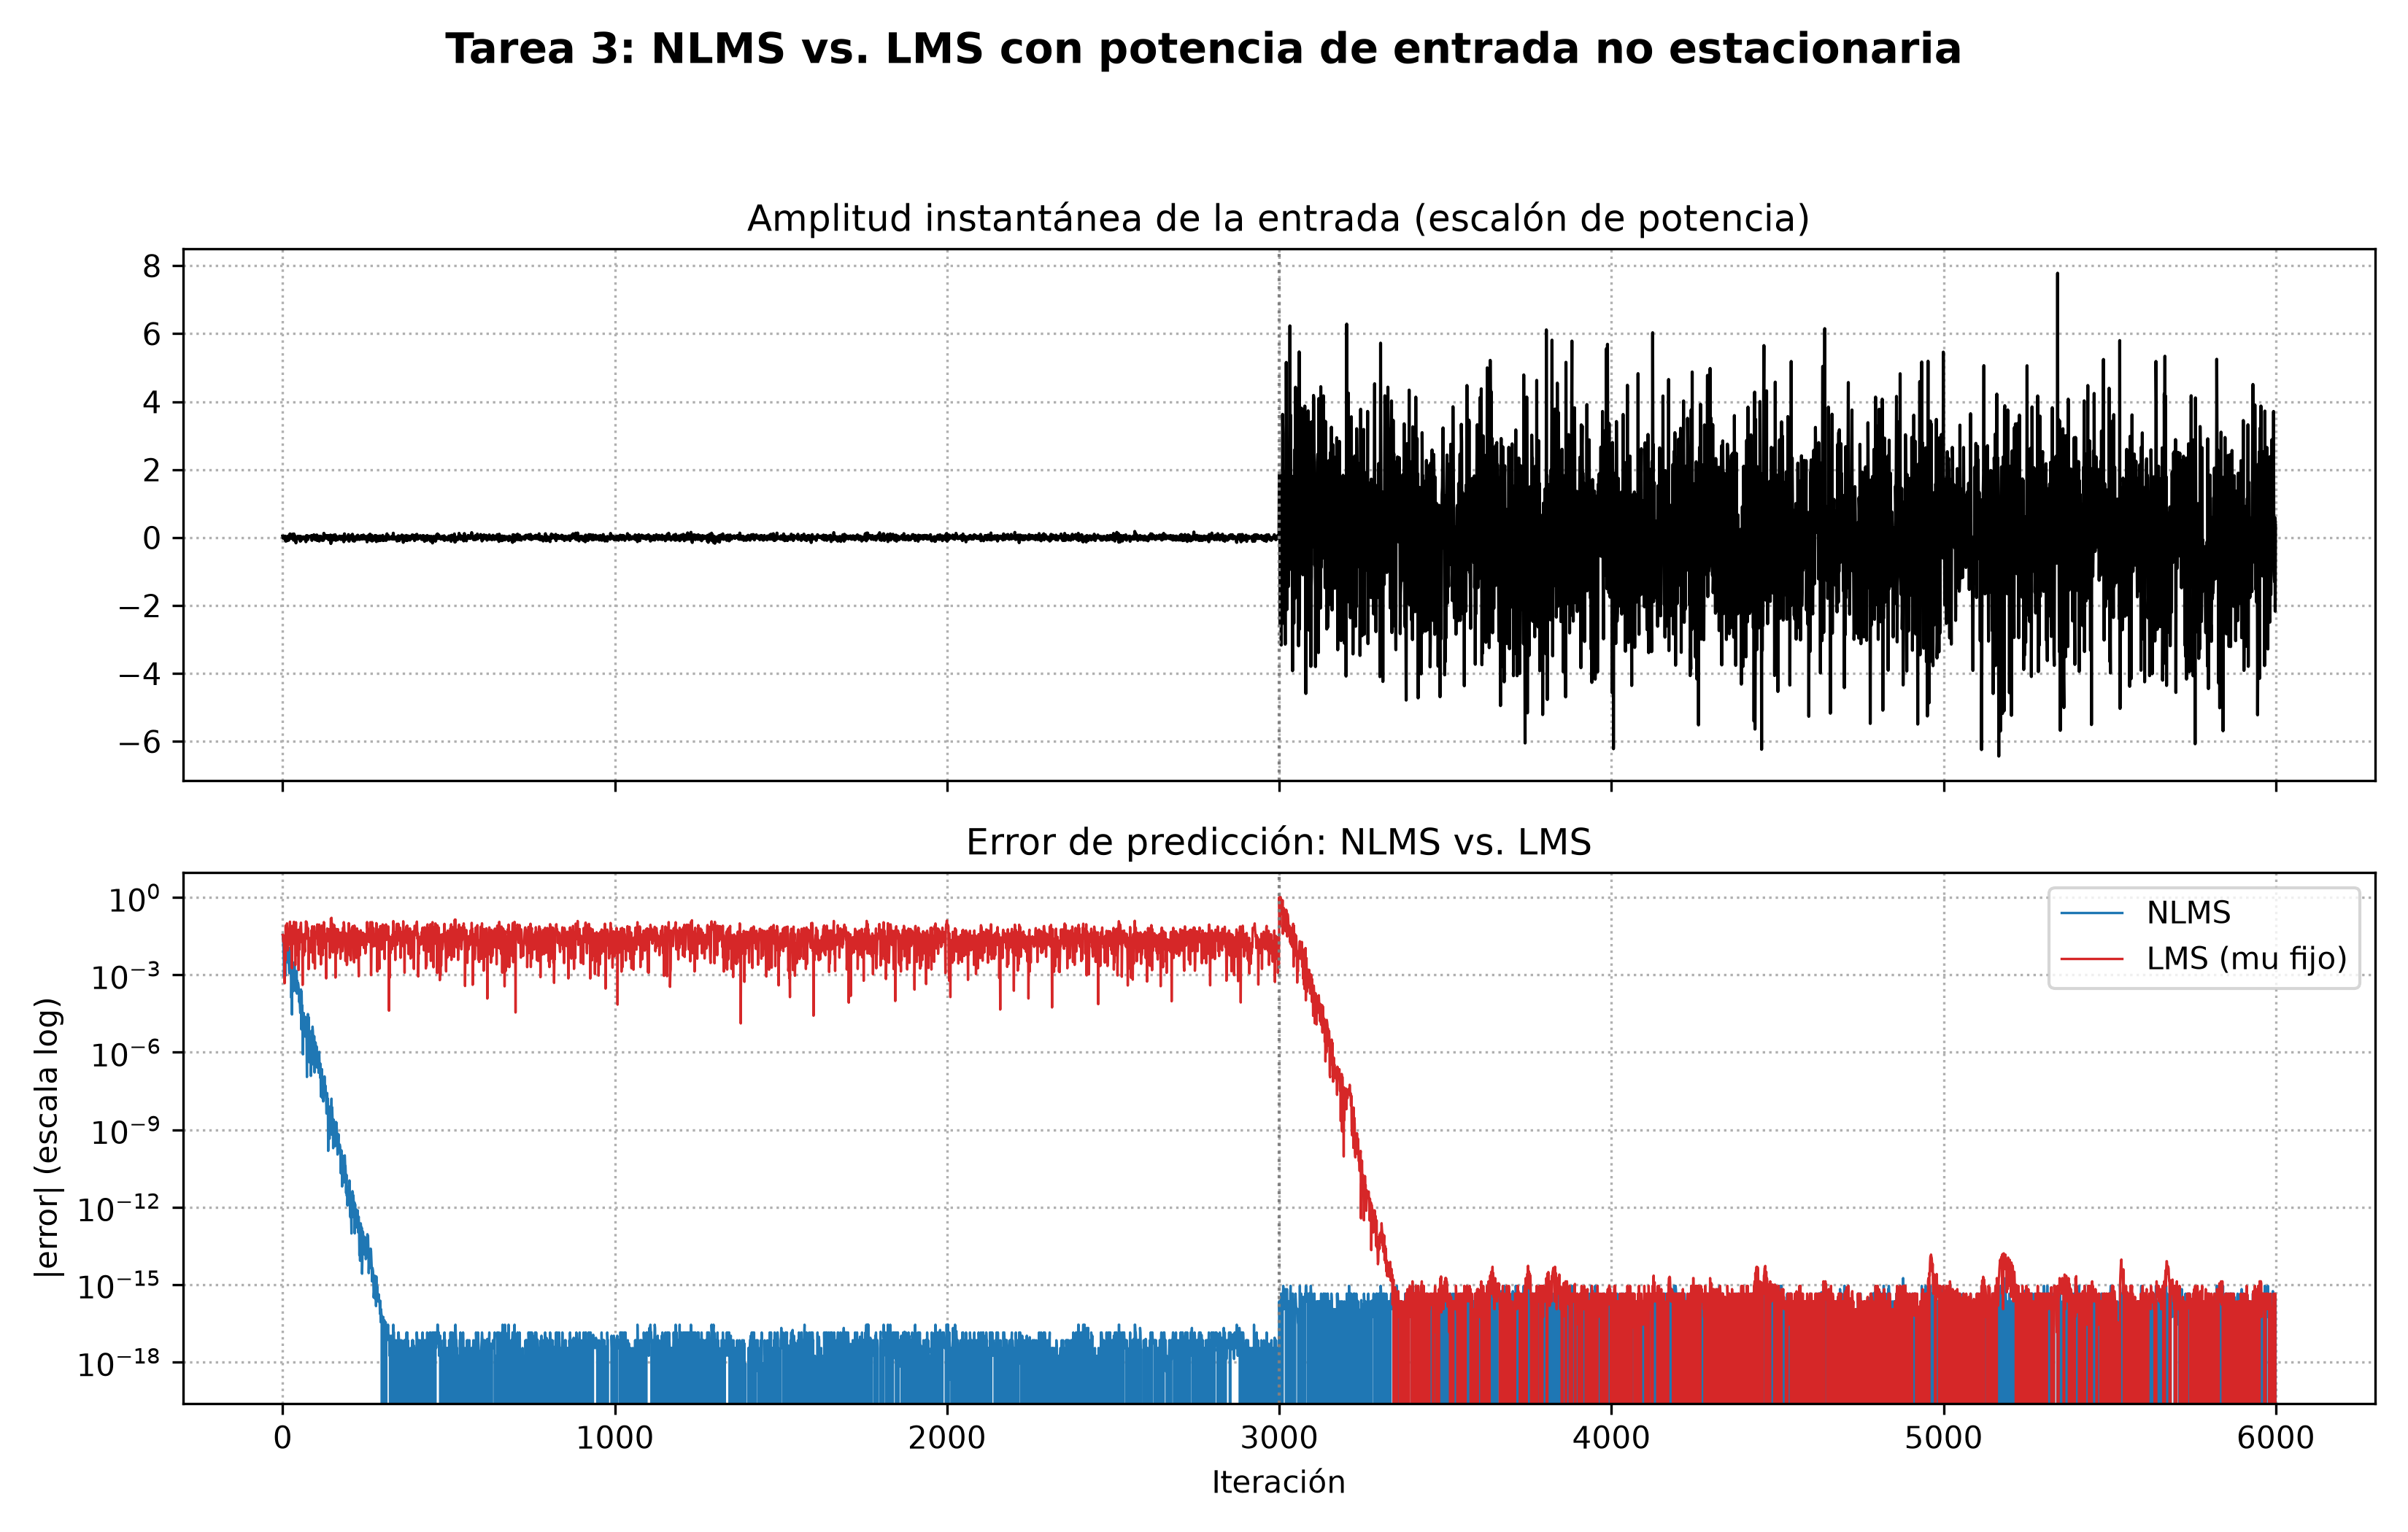
\includegraphics[width=\columnwidth]{work_twelve_t3_nlms_vs_lms_varying_power.png}
\caption{Comparación NLMS vs.\ LMS sobre una entrada con un cambio abrupto de potencia (factor 40) a mitad del experimento. El panel muestra el error de identificación de cada algoritmo en ambos segmentos, evidenciando que NLMS mantiene un error bajo y consistente en ambos mientras que LMS, con un $\mu$ fijo conservador, degrada su desempeño en el segmento de menor potencia.}
\label{fig:work_twelve_t3}
\end{figure}
